\apendice{Documentación técnica de programación}

\section{Introducción}

En este apartado se va a detallar la estructura del proyecto, las partes que lo componen y la función de cada una. El código final de la aplicación se encuentra dentro de \texttt{/SegundaFase}, el resto de directorios se mantienen como partes del repositorio(\url{https://github.com/etc99/algoritmosYmazmorras}) a modo de histórico de fases previas por las que ha pasado el proyecto antes de tomar la aproximación actual.

\section{Manual del programador}

El código del proyecto se divide entre dos partes principales; una para la aplicación de Unity, incluida en \texttt{/AlgoritmosYMazmorras}; y la parte del servidor de laberintos contenida en \texttt{/Mazmorras}.

\subsection{\texttt{/AlgoritmosYMazmorras}}
Este directorio contiene todo lo relativo a la aplicación de Unity. Sigue la estructura de un proyecto común de Unity.

\subsubsection{\texttt{/Assets}}
Contiene los recursos utilizados en el proyecto. En este directorio se encuentran los \textit{scripts} que establecen los comportamiento de los distintos componentes del juego. También contiene las escenas del juego, así como distintos recursos gráficos, de audio y de texturas utilizados en el juego. Además contiene los distintos \_Prefabs\_ creados para el proyecto.

\subsubsection{\texttt{/Packages}}
Contiene los paquetes utilizados por Unity para el proyecto. Normalmente no hay necesidad de modificar nada de este directorio debido a que el propio Unity ya lo gestiona.

\subsubsection{\texttt{/Library}}
En este directorio se encuentran los archivos generados por Unity en la compilación del juego. Este directorio no es necesario que tenga seguimiento por Git.

\subsubsection{\texttt{/ProjectSettings}}
Este directorio contiene la configuración del proyecto, así como configuración específica del editor de Unity.


\subsection{\texttt{/Mazmorras}}
En este directorio está contenido el servidor de Python junto con los distintos generadores de laberintos, así como de su persistencia en la base de datos de MongoDB.

También contiene ficheros Dockerfile y docker-compose con las que levantar la aplicación en un entorno de contenedores de Docker.

\subsubsection{\texttt{/.devcontainer}}
Esta carpeta contiene los archivos de configuración para el uso de la tecnología de los devcontainers. Está compuesto por un fichero Dockerfile para configurar la imagen del servidor a utilizar en el contenedor de desarrollo, un fichero \texttt{docker-compose.yml} que contiene la configuración con la que lanzar los distintos contenedores de la aplicación para el desarrollo y un fichero \texttt{devcontainer.json} con configuración propia de la tecnología de los devcontainers.

\subsubsection{\texttt{/src}}
Dentro de este directorio está contenido el código que compone el servidor de laberintos.

El fichero \texttt{requirements.txt} contiene las dependencias de bibliotecas externas de nuestro proyecto de Python.

El servidor del backend junto a sus endpoints están declarados dentro del fichero \texttt{app.py}. Desde aquí será donde se manejarán las peticiones realizadas al servidor.

Para lanzar el servidor más cómodamente utilizando uvicorn se ha creado un \textit{script} de nombre \texttt{main.py}.

\subsubsection{\texttt{/dungeon\_api}}

Es la carpeta con los componentes principales del funcionamiento del servidor.

El directorio \texttt{/dungeon\_controllers} contiene módulos que se encargan de la generación de los laberintos y su persistencia en la base de datos. Estos son utilizados en el manejo de peticiones del servidor.

El otro subdirectorio es \texttt{/dungeon\_generators}, que contienen los generadores de laberintos de cada uno de los algoritmos implementados. Para implementarlos se ha recurrido a un enfoque de programación orientada a objetos para añadir funcionalidades que faciliten su serialización y configuración. Todos los generadores heredan de \texttt{DungeonBase}, que provee una interfaz común para los generadores. Está contenido en \texttt{dungeon\_base.py}.

Para la gestión del almacenamiento en MongoDB de los laberintos se usan los modelos de \texttt{/models}. Los modelos definidos aquí dan la estructura que seguirán las entidades almacenadas en la base de datos.


\section{Compilación, instalación y ejecución del proyecto}
Para poder ejecutar este proyecto se tienen que preparar dos partes, el servidor y el cliente, en este caso Unity. En esta sección se va a explicar como preparar ambas partes para poder desarrollar el proyecto.

\subsection{Instalación de Unity}

Unity tiene soporte para ciertos sistemas operativos, entre ellos están
\begin{enumerate}
    \item Windows 7,8,10,11 
    \item macOs X 10.13+
    \item CentOS 7
    \item Rocky
    \item Ubuntu 18.04, 20.04, 22.04
\end{enumerate}

Para poder realizar la instalación del motor gráfico, primero se necesita realizar la descarga de Unity Hub. En el caso de Windows y macOS se necesitaría proceder con los siguientes pasos:
\begin{enumerate}
    \item Acceder a la web de Unity \url{https://unity.com/es/download}.
    \item Desde esa URL se descarga Unity Hub.
    \item Proceder con el proceso del instalador de la ventana de \texttt{setup}.
\end{enumerate}

Al abrir Unity Hub por primera vez, pide el inició de sesión con tu cuenta de Unity, si no se tiene una cuenta previamente se necesita crearla.
Tras esto, en la ventana de unity hub, en el menú de la derecha aparecen distintos botones, entre ellos el botón de <<Installs>> donde aparecerá automáticamente el inicio de descarga de Unity como se muestra en la figura \ref{fig:InstallsUnity}.

\begin{figure}[!h]  
    \centering  
    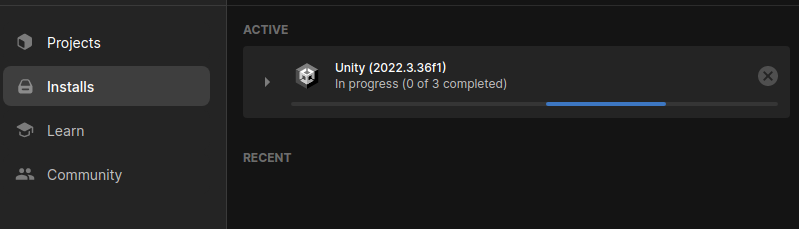
\includegraphics[width=\textwidth]{img/InstallsUnity.png}  
    \caption{Pestaña de instalación de Unity en UnityHub.}  
    \label{fig:InstallsUnity}
\end{figure}

Es recomendable para poder visualizar y trabajar con los \textit{scripts} de Unity instalar Visual Studio Community
Tras la instalación anterior se puede realizar desde el Unity, Edit>Preferences y desde ahí se cambia la herramienta externa.

Tras esto solo quedaría exportar el proyecto a Unity. Unity va a pedir que se instale una versión previa y es porque este proyecto se hizo con la versión \texttt{2021.3.25f1}. 
\begin{figure}[!h]  
    \centering  
    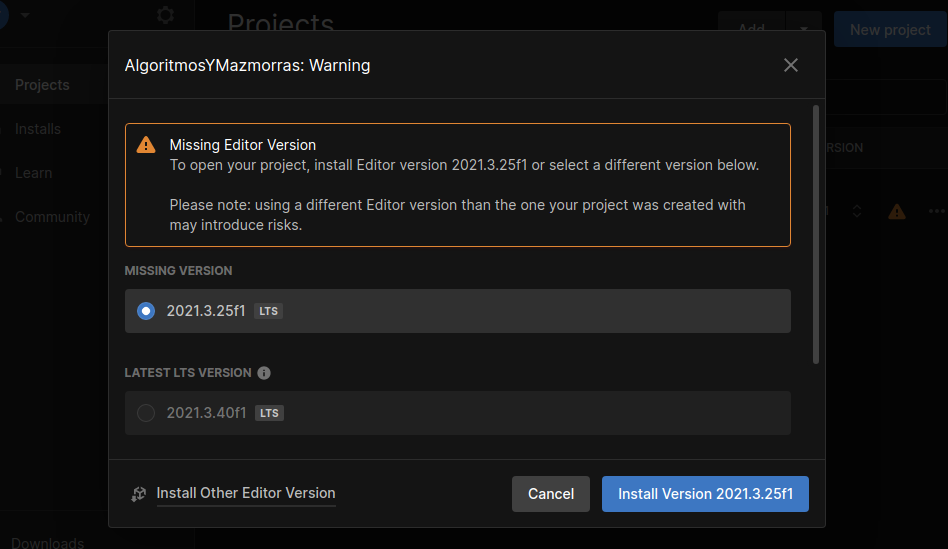
\includegraphics[width=\textwidth]{img/UnityInstallVersion.png}  
    \caption{Pestaña de instalación de nueva versión en Unity.}  
    \label{fig:UnityInstallVersion}
\end{figure}

\subsection{Instalación de Docker}

Para instalar docker primero se necesita obtener de la página de descargas, se puede escoger la versión del siguiente enlace \url{https://docs.docker.com/desktop/release-notes/} y se obtendrá el instalador.
Tras esto sólo quedaría seguir los pasos del instalador. Tras la instalación se necesita ejecutar con permisos administrador.

En máquinas con Windows, es necesario habilitar WSL~\cite{wslContainers}, el subsistema Linux para Windows, para realizarlo se puede hacer desde Docker, como se muestra en la figura \ref{fig:dockerdashboard}.

\begin{figure}[!h]  
    \centering  
    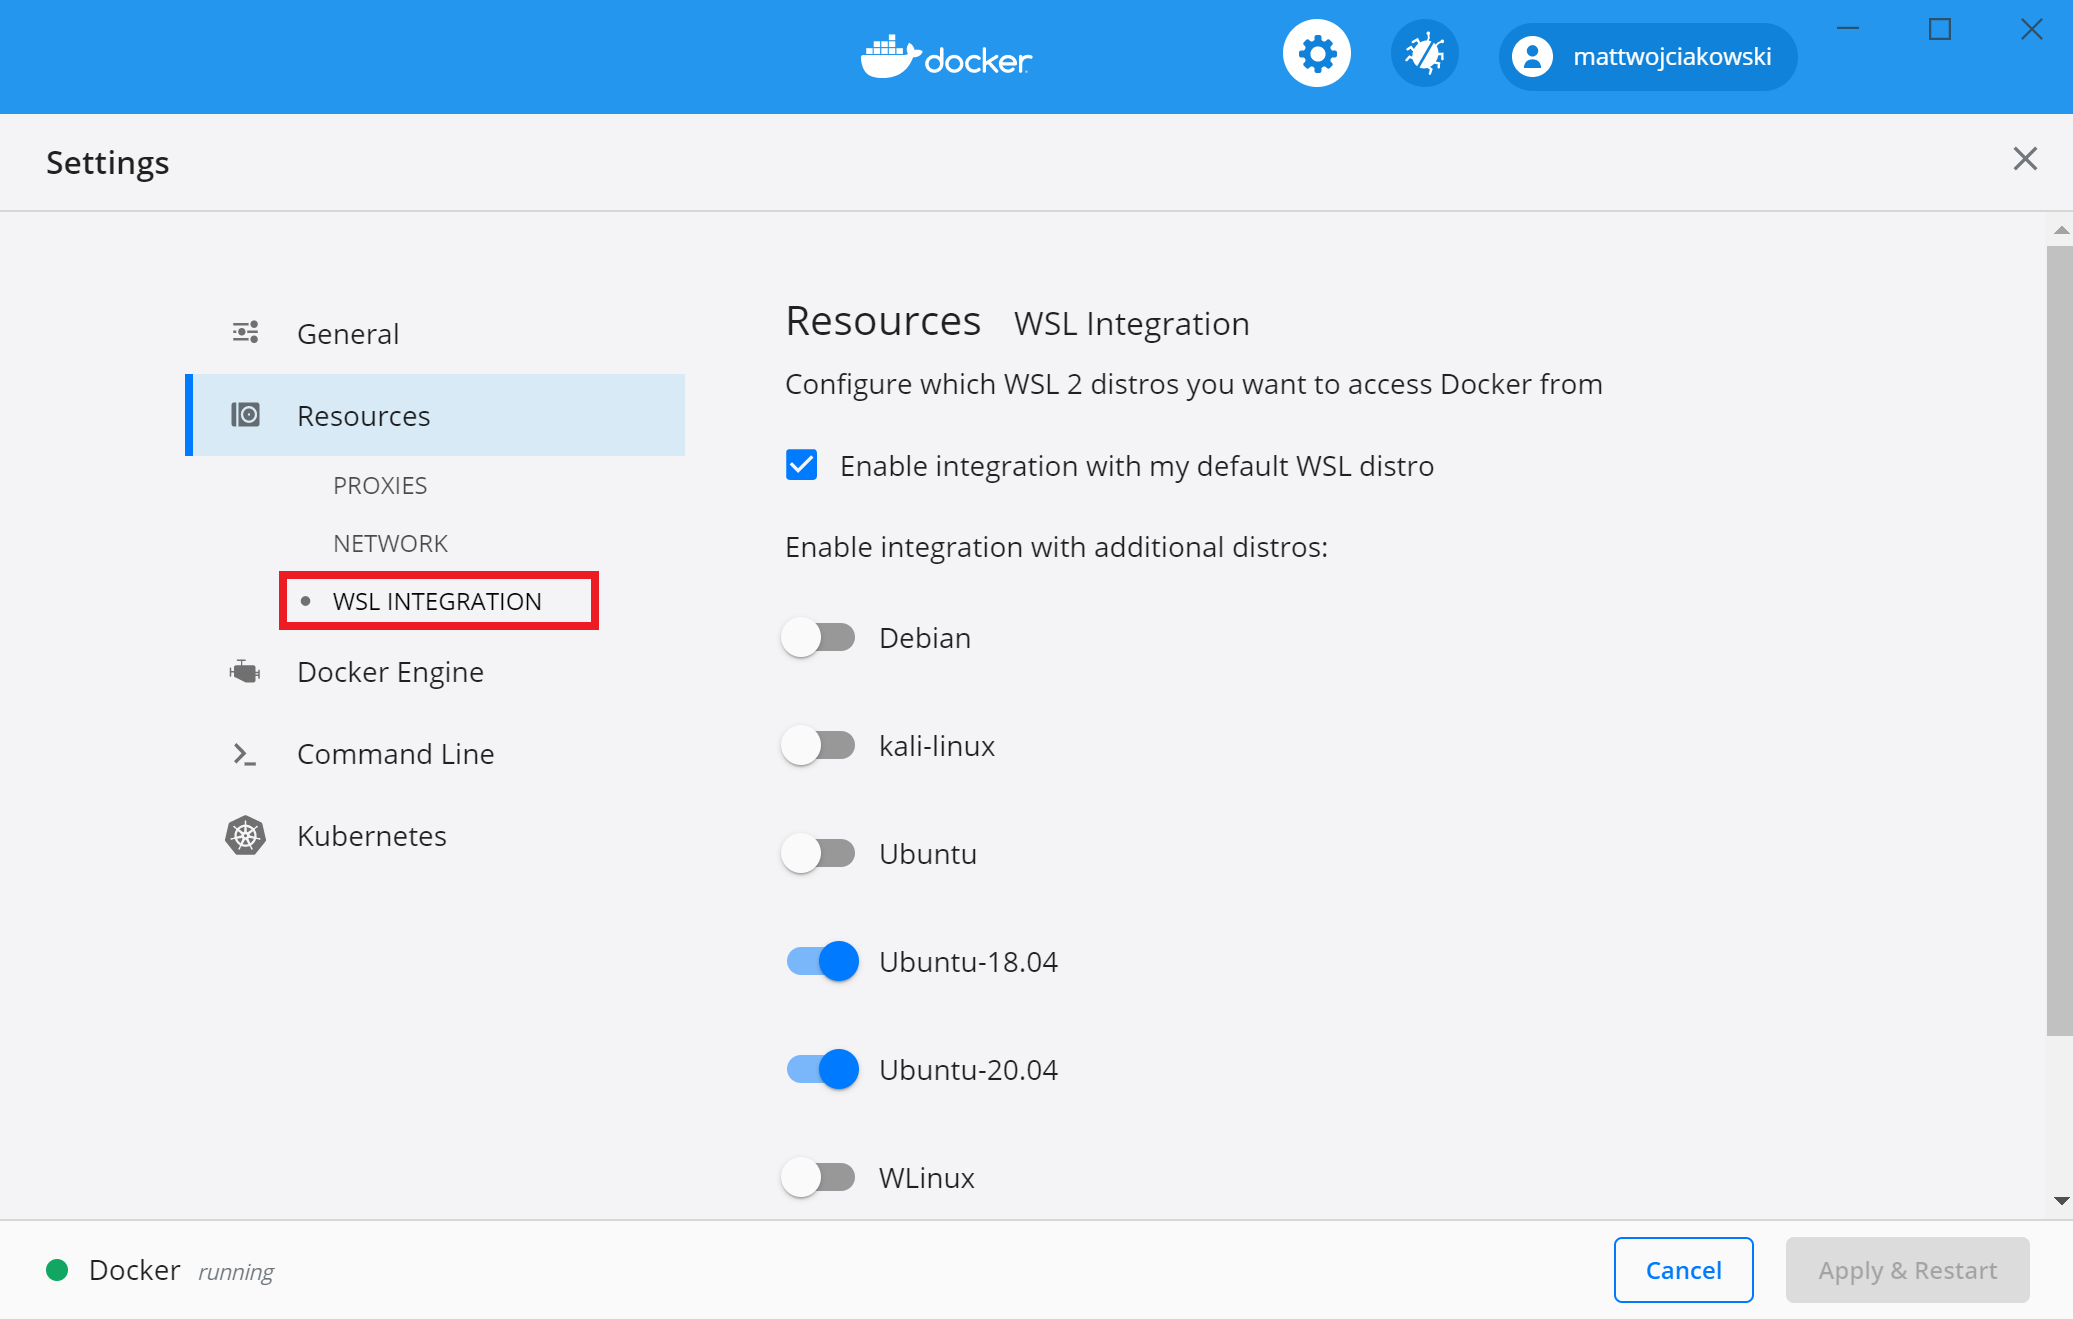
\includegraphics[width=\textwidth]{img/docker-dashboard.png}  
    \caption{Ventana de docker para habilitar WSL. Imagen extraída de \url{https://learn.microsoft.com/es-es/windows/wsl/tutorials/wsl-containers}}  
    \label{fig:dockerdashboard}
\end{figure}


\subsection{Preparación de DevContainer}

Desde Visual Studio Code se puede abrir el contenido del proyecto correspondiente a la carpeta \texttt{/Mazmorras}. Para hacerlo en la esquina superior derecha como se muestra en la figura \ref{fig:FileVS}.

Una vez abierto se necesita descargar la extensión \texttt{Dev Containers}. Para hacerlo en la barra de menú que se encuentra en el margen derecho se debe ir al botón que se muestra en la figura \ref{fig:Extensiones}.
La extensión es la que se muestra en la figura \ref{fig:DevContainers}.

\begin{figure}[!h]  
    \centering  
    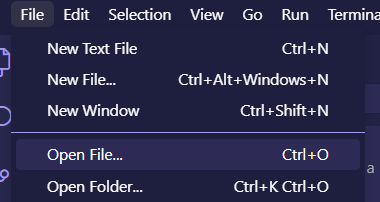
\includegraphics[width=\textwidth]{img/FileVS.png}  
    \caption{Pestaña de archivos en Visual Studio Code}  
    \label{fig:FileVS}
\end{figure}
\begin{figure}[!h]  
    \centering  
    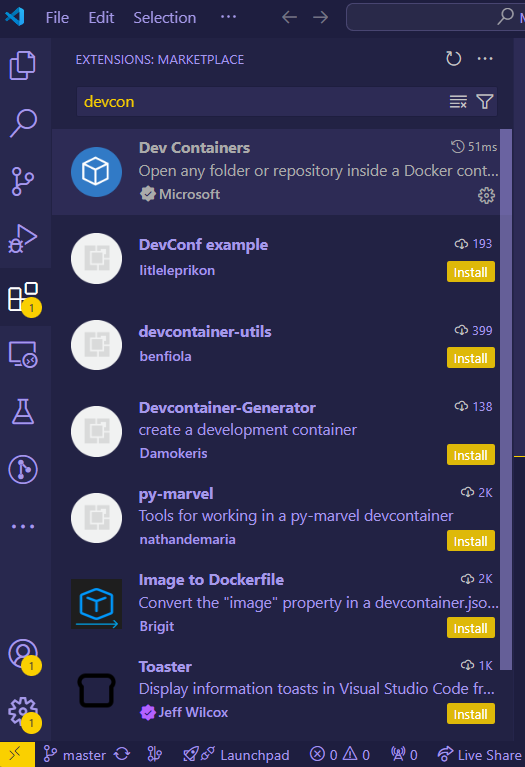
\includegraphics[width=\textwidth]{img/Extensiones.png}  
    \caption{Pestaña extensiones en Visual Studio Code}  
    \label{fig:Extensiones}
\end{figure}
\begin{figure}[!h]  
    \centering  
    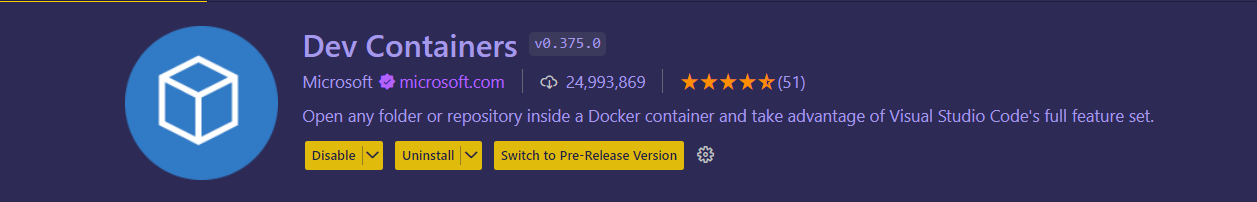
\includegraphics[width=\textwidth]{img/devcontainersextension.png}  
    \caption{Pestaña de la extensión Dev Containers en Visual Studio Code}  
    \label{fig:DevContainers}
\end{figure}

Al instalar la extensión, automáticamente aparece la notificación de la figura \ref{fig:opencontainer}, al pulsar en el botón de <<Reopen in container>> volverá a abrir el proyecto, esta vez desde el contenedor ya preparado.

\begin{figure}[!h]  
    \centering  
    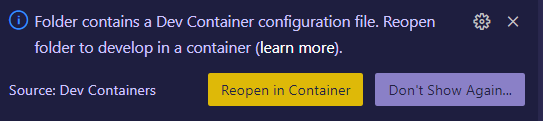
\includegraphics[width=\textwidth]{img/reopencontainer.png}  
    \caption{Notificación de reapertura de proyecto como Dev Container}  
    \label{fig:opencontainer}
\end{figure}

Si no apareciese la notificación, se puede abrir con la extensión siguiendo los siguientes pasos. Primero se necesita pulsar el botón para abrir el proyecto desde una ventana remota, como se muestra en la figura \ref{fig:botoncontainer}. Tras esto se abrirá el menú de selección como se muestra en la figura \ref{fig:remoteWindow}. Se necesita seleccionar la opción <<Reopen in Container>>, al hacerlo se volverá a abrir el proyecto desde el contenedor.

\begin{figure}[!h]  
    \centering  
    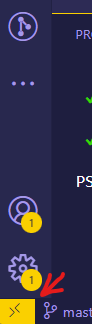
\includegraphics{img/botoncontainer.png}  
    \caption{Botón para ejecutar la apertura de una ventana remota}  
    \label{fig:botoncontainer}
\end{figure}

\begin{figure}[!h]  
    \centering  
    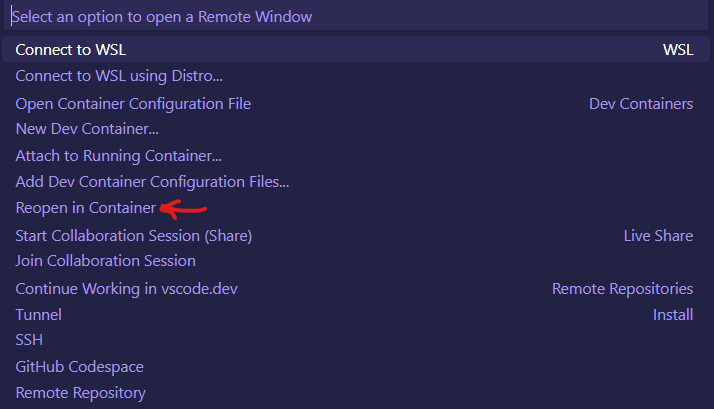
\includegraphics[width=\textwidth]{img/reopencontainerdevcontainer.png}  
    \caption{Menú de ejecución de ventana remota}  
    \label{fig:remoteWindow}
\end{figure}

\subsection{Levantar el servidor}

Para levantar el servidor se aconseja usar la terminal integrada de Visual Studio Code, esta se puede abrir desde la barra superior de la ventana como se muestra en la figura \ref{fig:terminal}.
\begin{figure}[!h]  
    \centering  
    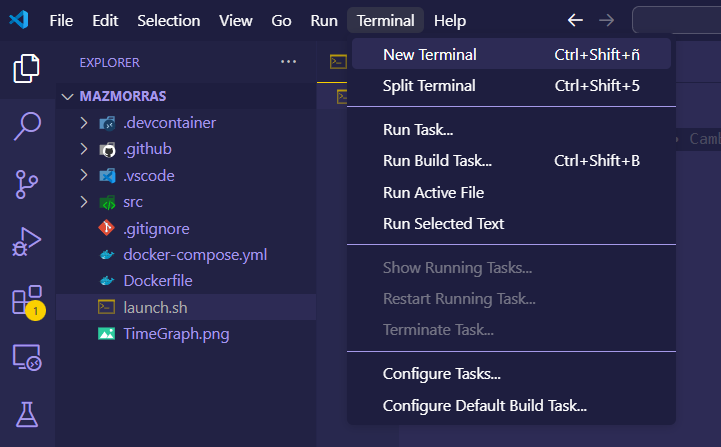
\includegraphics[width=\textwidth]{img/terminal.png}  
    \caption{Barra de opciones de Visual Studio Code}  
    \label{fig:terminal}
\end{figure}

El servidor de laberintos se lanza a través de un contendor de Docker, siguiendo la configuración especificada en el Dockerfile. Para poder hacerlo tenemos que introducir en la terminal en la ruta del directorio del backend el siguiente comando: 
\begin{lstlisting}
    docker compose up
\end{lstlisting}
Se lanzarán un contenedor con el servidor y otro de mongo, siguiendo la configuración del fichero Docker-compose.yml contenida en ese directorio.

Para poder parar el contenedor, desde el teclado se pulsarían los botones Ctrl+C y para borrar el contenedor se realiza con el siguiente comando:
\begin{lstlisting}
    docker compose down
\end{lstlisting}



\section{Pruebas del sistema}
Es necesario para asegurar una buena experiencia de usuario poner el sistema desarrollado a prueba. En el caso de este proyecto, está compuesto de dos partes que necesitan pruebas distintas.

Para realizar pruebas que comprueben el funcionamiento del servidor, se realizaron pruebas de peticiones predefinidas y respuestas esperadas, en este caso la herramienta elegida fue Postman\footnote{Esta herramienta permite comprobar el correcto funcionamiento de una API a través de llamadas predefinidas, para más información \url{https://learning.postman.com/docs/introduction/overview/}}.

Para comprobar el correcto funcionamiento del videojuego, se han preparado ejecutables que después se han testeado, a este proceso se le llama beta testeo. Se recomienda que este testeo lo realicen personas no familiarizadas con el proyecto, estas probarán el videojuego para poder encontrar problemas que el desarrollador no podría encontrar. El proceso de beta testeo fue esencial para obtener una experiencia de usuario adecuada.

